\documentclass[aspectratio=169]{beamer}

\usepackage{ccicons}
\usepackage{fontspec}
\usepackage{import}
\usepackage{listings}
\usepackage{tikz}

\subimport{../}{colors.tex}

\usetikzlibrary{
  arrows,
  arrows.meta,
  automata,
  backgrounds,
  calc,
  chains,
  decorations.pathreplacing,
  fit,
  matrix,
  overlay-beamer-styles,
  positioning,
  shapes,
  tikzmark,
}
\usetikzmarklibrary{listings}

\hypersetup{
  colorlinks=true,
  urlcolor=uclablue,
}

\setbeamercolor{frametitle}{fg=primarycolor}
\setbeamercolor{structure}{fg=primarycolor}
\setbeamercolor{enumerate item}{fg=black}
\setbeamercolor{itemize item}{fg=black}
\setbeamercolor{itemize subitem}{fg=black}

\setbeamersize{text margin left=26.6mm}
\addtolength{\headsep}{2mm}

\setbeamertemplate{navigation symbols}{}
\setbeamertemplate{headline}{}
\setbeamertemplate{footline}{}
\setbeamertemplate{itemize item}{\color{black}}
\setbeamertemplate{itemize items}[circle]

\setbeamertemplate{footline}{
  \begin{tikzpicture}[remember picture,
                      overlay,
                      shift={(current page.south west)}]
    \node [black!50, inner sep=2mm, anchor=south east]
          at (current page.south east) {\footnotesize \insertframenumber};
  \end{tikzpicture}
}

\setsansfont{Overpass}[Scale=MatchLowercase]
\setmonofont{Overpass Mono}[Scale=MatchLowercase]

\makeatletter
\newcommand\version[1]{\renewcommand\@version{#1}}
\newcommand\@version{}
\def\insertversion{\@version}

\newcommand\lecturenumber[1]{\renewcommand\@lecturenumber{#1}}
\newcommand\@lecturenumber{}
\def\insertlecturenumber{\@lecturenumber}
\makeatother

\setbeamertemplate{title page}
{
  \begin{tikzpicture}[remember picture,
                      overlay,
                      shift={(current page.south west)},
                      background rectangle/.style={fill=uclablue},
                      show background rectangle]
    \node [anchor=west, align=left, inner sep=0, text=white]
          (lecturenumber) at (\paperwidth / 6, \paperheight * 3 / 4)
          {\Large Lecture \insertlecturenumber};
    \node [inner sep=0, align=left, text=white, node distance=0,
           above left=of lecturenumber, anchor=south west, yshift=2mm]
          {\Large CS 111: Operating System Principles};
    \node (title) [inner sep=0, anchor=west, align=right, text=white]
          at (\paperwidth / 6, \paperheight / 2)
          {{\bfseries \Huge \inserttitle{}}};
    \node [inner sep=0, align=right, text=white, node distance=0,
           below right=of title, anchor=north east, yshift=-1mm]
          {{\footnotesize \ttfamily \insertversion}};
    \node [inner sep=0, text=white, align=left, anchor=west]
          (author) at (\paperwidth / 6, \paperheight / 4)
          {\insertauthor};
    \node [text=white, inner sep=0, align=left, node distance=0,
           below left=of author, anchor=north west, yshift=-2mm]
          {\insertdate};
    \node [align=right, anchor=south east, inner sep=2mm, text=white]
          (license) at (\paperwidth, 0)
          {\footnotesize This  work is licensed under a
           \href{http://creativecommons.org/licenses/by-sa/4.0/}
                {\color{uclagold} Creative Commons Attribution-ShareAlike 4.0
                 International License}};
    \node [text=white, inner sep=0, align=right, node distance=0,
           above right=of license, anchor=south east, xshift=-2mm]
          {\Large \ccbysa};
  \end{tikzpicture}
}

\tikzset{
  >=Straight Barb[],
  shorten >=1pt,
  initial text=,
}

\lstset{
  basicstyle=\footnotesize\ttfamily,
}


\lecturenumber{8}
\title{Advanced Scheduling}
\version{1.0.0}
\author{Jon Eyolfson}
\date{April 15, 2021}

\begin{document}
  \begin{frame}[plain, noframenumbering]
    \titlepage
  \end{frame}

  \begin{frame}
    \frametitle{We Could Add Priorities}

    We may favor some processes over others

    \hspace{2em} Assign each process a priority

    \vspace{2em}

    Run higher priority processes first, round-robin processes of equal priority

    \hspace{2em} Can be preemptive or non-preemptive
  \end{frame}

  \begin{frame}
    \frametitle{Priorities Can Be Assigned an Integer}
    
    We can pick a lower, or higher number, to mean high priority

    \hspace{2em} In Linux -20 is the highest priority, 19 is the lowest

    \vspace{2em}

    We may lead processes to \textit{starvation} if there's a lot of higher
    priority processes

    \vspace{2em}

    One solution is to have the OS dynamically change the priority

    \hspace{2em} Older processes that haven't been executed in a long time increase priority
  \end{frame}

  \begin{frame}
    \frametitle{Priority Inversion is a New Issue}

    We can accidentally change the priority of a low priority process to a high one

    \hspace{2em} This is caused by dependencies, e.g. a high priority depends a low priority

    \vspace{2em}

    One solution is \textit{priority inheritance}

    \hspace{2em} Inherit the highest priority of the waiting processes

    \hspace{2em} Chain together multiple inheritances if needed

    \hspace{2em} Revert back to the original priority after dependency
  \end{frame}

  \begin{frame}
    \frametitle{A Foregound Process Can Recieve User Input, Background Can Not}

    Unix background process when: process group ID differs from its terminal group ID

    \hspace{2em} You do not need to know this specific definition

    \vspace{2em}

    The idea is to separate processes that users interact with:

    \hspace{2em} Foreground processes are interactable and need good response time

    \hspace{2em} Background processes may not need good response time, just throughput
  \end{frame}

  \begin{frame}
    \frametitle{We Can Use Multiple Queues for Other Purposes}

    We could create different queues for foreground and background processes:

    \hspace{2em} Foreground uses RR

    \hspace{2em} Background uses FCFS

    \vspace{2em}

    Now we have to schedule between queues!

    \hspace{2em} RR between the queues

    \hspace{2em} Use a priority for each queue
  \end{frame}

  \begin{frame}
    \frametitle{Scheduling Can Get Complicated}

    There's no ``right answer'', only trade-offs

    \vspace{2em}

    We haven't talked about multiprocessor scheduling yet

    \vspace{2em}

    We'll assume symmetric multiprocessing

    \hspace{2em} All CPUs are connected to the same physical memory

    \hspace{2em} The CPUs have their own private cache (at least the lowest levels)
  \end{frame}

  \begin{frame}
    \frametitle{One Approach is to Use the Same Scheduling for All CPUs}

    There's still only one scheduler

    \hspace{2em} It just keeps adding processes while there's available CPUs

    \vspace{2em}

    Advantages

    \hspace{2em} Good CPU utilization

    \hspace{2em} Fair to all processes

    \vspace{2em}

    Disadvantages

    \hspace{2em} Not scalable (everything blocks on global scheduler)

    \hspace{2em} Poor cache locality

    \vspace{2em}

    This was the approach in Linux 2.4
  \end{frame}

  \begin{frame}
    \frametitle{We Can Create Per-CPU Schedulers}

    When there's a new process, assign it to a CPU

    \hspace{2em} One strategy is to assign it to the CPU with the lowest number of processes

    \vspace{2em}

    Advantages

    \hspace{2em} Easy to implement

    \hspace{2em} Scalable (there's no blocking on a resource)

    \hspace{2em} Good cache locality

    \vspace{2em}

    Disadvantages

    \hspace{2em} Load imbalance

    \hspace{4em} Some CPUs may have less processes, or less intensive ones
  \end{frame}

  \begin{frame}
    \frametitle{We Can Compromise between Global and Per-CPU}

    Keep a global scheduler that can rebalance per-CPU queues

    \hspace{2em} If a CPU is idle, take a process from another CPU (work stealing)

    \vspace{2em}

    You may want more control over which processes can switch

    \hspace{2em} Some may be more sensitive to caches

    \vspace{2em}

    Use \textit{processor affinity}

    \hspace{2em} The preference of a process to be scheduled on the same core

    \vspace{2em}

    This is a simplified version of the O(1) scheduler in Linux 2.6
  \end{frame}

  \begin{frame}
    \frametitle{Another Strategy is ``Gang'' Scheduling}

    Multiple processes may need to be scheduled simultaneously

    \vspace{2em}

    The scheduler on each CPU cannot be completely independent

    \vspace{2em}

    ``Gang Scheduling'' (Coscheduling)

    \hspace{2em} Allows you to run a set of processes simultaneously (acting as a unit)

    \vspace{2em}

    This requires a global context-switch across all CPUs
  \end{frame}

  \begin{frame}
    \frametitle{Real-Time Scheduling is Yet Another Problem}

    Real-time means there are time constraints, either for a deadline or rate

    \hspace{2em} e.g. audio, autopilot

    \vspace{2em}

    A hard real-time system

    \hspace{2em} Required to guarantee a task completes within a certain amount
    of time

    \vspace{2em}

    A soft real-time system

    \hspace{2em} Critical processes have a higher priority and the deadline is
    met in practice

    \vspace{2em}

    Linux is an example of soft real-time
  \end{frame}

  \begin{frame}
    \frametitle{Linux Also Implements FCFS and RR Scheduling}

    You can search around in the source tree: FCFS (\texttt{SCHED\_FIFO} and RR (\texttt{SCHED\_RR})

    \vspace{2em}

    Use a multilevel queue scheduler for processes with the same priority

    \hspace{2em} Also let the OS dynamically adjust the priority

    \vspace{2em}

    Soft real-time processes:

    \hspace{2em} Always schedule the highest priority processes first

    Normal processes:

    \hspace{2em} Adjust the priority based on aging
  \end{frame}

  \begin{frame}
    \frametitle{Real-Time Processes Are Always Prioritized}

    The soft real-time scheduling policy will either be \texttt{SCHED\_FIFO}
    or \texttt{SCHED\_RR}

    \hspace{2em} There are 100 static priority levels (1---99)

    \vspace{2em}

    Normal scheduling policies apply to the other processes
    (\texttt{SCHED\_NORMAL})

    \hspace{2em} By default the priority is 0

    \hspace{2em} Priority ranges from $\mathsf{[-20, 19]}$

    \hspace{2em}

    Processes can change their own priorities with system calls:

    \hspace{2em} \texttt{nice}, \texttt{sched\_setscheduler}
  \end{frame}

  \begin{frame}
    \frametitle{Linux Scheduler Evolution}

    2.4---2.6, a $\mathsf{O(N)}$ global queue

    \hspace{2em} Simple, but poor performance with multiprocessors and many processes

    \vspace{2em}

    2.6---2.6.22, a per-CPU run queue, $\mathsf{O(1)}$ scheduler

    \hspace{2em} Complex to get right, interactivity had issues

    \hspace{2em} No guarantee of fairness

    \vspace{2em}

    2.6.23---Present, the completely fair scheduler (CFS)

    \hspace{2em} Fair, and allows for good interactivity
  \end{frame}

  \begin{frame}
    \frametitle{The $\mathsf{O(1)}$ Scheduler Has Issues with Modern Processes}

    Foreground and background processes are a good division

    \hspace{2em} Easier with a terminal, less so with GUI processes

    \vspace{2em}

    Now the kernel has to detect interactive processes with heuristics

    \hspace{2em} Processes that sleep a lot may be more interactive

    \hspace{4em} This is ad hoc, and could be unfair

    \vspace{2em}

    How would we introduce fairness for different priority processes?

    \hspace{2em} Use different size time slices

    \hspace{2em} The higher the priority, the larger the time slice

    \hspace{4em} There are also situations where this ad hoc solution could be unfair
  \end{frame}

  \begin{frame}
    \frametitle{Ideal Fair Scheduling}

    Assume you have an infinitely small time slice

    \hspace{2em} If you have $\mathsf{n}$ processes, each runs at $\mathsf{\frac{1}{n}}$ rate

    \vspace{2em}

    \begin{tikzpicture}
      \draw (0, 6em) rectangle (30em, 7.5em);

      \node [anchor=east] at (0, 6.75em) {1 Process};

      \draw (0, 3.5em) rectangle (10em, 5em);
      \draw (0, 1.75em) rectangle (10em, 3.25em);
      \draw (0, 0) rectangle (10em, 1.5em);

      \node [anchor=east] at (0, 2.5em) {3 Processes};
    \end{tikzpicture}

    \vspace{2em} CPU usage is divided equally among every process
  \end{frame}

  \begin{frame}
    \frametitle{Example IFS Scheduling}

    Consider the following processes:
    \begin{center}
      \footnotesize
      \begin{tabular}{lrr}
        Process & Arrival Time & Burst Time \\
        $\mathsf{P_1}$ & 0 & 8 \\
        $\mathsf{P_2}$ & 0 & 4 \\
        $\mathsf{P_3}$ & 0 & 16 \\
        $\mathsf{P_4}$ & 0 & 4 \\
      \end{tabular}
    \end{center}

    Assume that each vertical slice can execute 4 time units.

    \hspace{2em} Each box represents the time units spend executing

    \begin{center}
      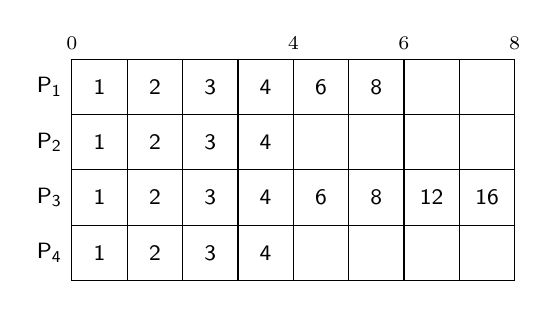
\begin{tikzpicture}

        %% \fill [black!80] (0,0) rectangle (14em, 2em);

        %% \fill [black!60] (14em,0) rectangle (22em, 2em);

        %% \fill [black!40] (22em,0) rectangle (24em, 2em);

        %% \fill [black!20] (24em,0) rectangle (32em, 2em);

        \draw (0,0) rectangle (16em,8em);

        \foreach \i in {1,...,7} {
          \draw [shorten >=0] (\i * 2em, 0) -- (\i * 2em, 8em);
        }

        \foreach \i in {1,...,3} {
          \draw [shorten >=0] (0, \i * 2em) -- (16em, \i * 2em);
        }

        \node [anchor=east] at (0, 7em) {\footnotesize $\mathsf{P_1}$};
        \node [anchor=east] at (0, 5em) {\footnotesize $\mathsf{P_2}$};
        \node [anchor=east] at (0, 3em) {\footnotesize $\mathsf{P_3}$};
        \node [anchor=east] at (0, 1em) {\footnotesize $\mathsf{P_4}$};

        \node at (1em, 7em) {\footnotesize $\mathsf{1}$};
        \node at (1em, 5em) {\footnotesize $\mathsf{1}$};
        \node at (1em, 3em) {\footnotesize $\mathsf{1}$};
        \node at (1em, 1em) {\footnotesize $\mathsf{1}$};

        \node at (3em, 7em) {\footnotesize $\mathsf{2}$};
        \node at (3em, 5em) {\footnotesize $\mathsf{2}$};
        \node at (3em, 3em) {\footnotesize $\mathsf{2}$};
        \node at (3em, 1em) {\footnotesize $\mathsf{2}$};

        \node at (5em, 7em) {\footnotesize $\mathsf{3}$};
        \node at (5em, 5em) {\footnotesize $\mathsf{3}$};
        \node at (5em, 3em) {\footnotesize $\mathsf{3}$};
        \node at (5em, 1em) {\footnotesize $\mathsf{3}$};

        \node at (7em, 7em) {\footnotesize $\mathsf{4}$};
        \node at (7em, 5em) {\footnotesize $\mathsf{4}$};
        \node at (7em, 3em) {\footnotesize $\mathsf{4}$};
        \node at (7em, 1em) {\footnotesize $\mathsf{4}$};

        \node at (9em, 7em) {\footnotesize $\mathsf{6}$};
        \node at (9em, 3em) {\footnotesize $\mathsf{6}$};

        \node at (11em, 7em) {\footnotesize $\mathsf{8}$};
        \node at (11em, 3em) {\footnotesize $\mathsf{8}$};

        \node at (13em, 3em) {\footnotesize $\mathsf{12}$};

        \node at (15em, 3em) {\footnotesize $\mathsf{16}$};

        \node [anchor=south] at (0em, 8em) {\scriptsize 0};
        \node [anchor=south] at (8em, 8em) {\scriptsize 4};
        \node [anchor=south] at (12em, 8em) {\scriptsize 6};
        \node [anchor=south] at (16em, 8em) {\scriptsize 8};
      \end{tikzpicture}
    \end{center}
  \end{frame}

  \begin{frame}
    \frametitle{IFS is the Fairest but Impractical Policy}

    This policy is fair, every process gets an equal amount of CPU time

    \hspace{2em} Boosts interactivity, has the ideal response time

    \vspace{2em}

    However, this would perform way too many context switches

    \vspace{2em}

    You have to constantly scan all processes, which is $\mathsf{O(N)}$
  \end{frame}

  \begin{frame}
    \frametitle{Completely Fair Scheduler (CFS)}

    For each runnable process, assign it a ``virtual runtime''

    \hspace{2em} At each scheduling point where the process runs for time \texttt{t}

    \hspace{4em} Increase the virtual runtime by \texttt{t} $\mathsf{\times}$ weight (based on priority)

    \vspace{2em}

    The virtual runtime monotonically increases

    \hspace{2em} Scheduler selects the process based on the lowest virtual runtime

    \hspace{4em} Compute its dynamic time slice based on the IFS

    \vspace{2em}

    Allow the process to run, when the time slice ends repeat the process
  \end{frame}
  
  \begin{frame}
    \frametitle{CFS is Implemented with Red-Black Trees}

    A red-black tree is a self-balancing binary search tree

    \hspace{2em} Keyed by virtual runtime

    \hspace{4em} $\mathsf{O(lg N)}$ insert, delete, update

    \hspace{4em} $\mathsf{O(1)}$ find minimum

    \vspace{2em}

    The implementation uses a red-black tree with nanosecond granularity

    \hspace{2em} Doesn't need to guess the interactivity of a process

    \vspace{2em}

    CFS tends to favour I/O bound processes by default

    \hspace{2em} Small CPU bursts translate to a low virtual runtime

    \hspace{4em} It will get a larger time slice, in order to catch up to the ideal
  \end{frame}

  \begin{frame}
    \frametitle{Scheduling Gets Even More Complex}

    There are more solutions, and more issues:
    \begin{itemize}
      \item Introducing priority also introduces priority inversion
      \item Some processes need good interactivity, others not so much
      \item Multiprocessors may require per-CPU queues
      \item Real-time requires predictability
      \item Completely Fair Scheduler (CFS) tries to model the ideal fairness
    \end{itemize}
  \end{frame}
\end{document}
